%%%%%%%%%%%%%%%%%%%%%%%%%%%%%%%%%%%%%%%%%%%%%%%%%%%%%%%%%%%%%%%%%%%%%%%%%%%%%%%%%%
\begin{frame}[fragile]\frametitle{}

\begin{center}
{\Large Need}
\end{center}
\end{frame}

%%%%%%%%%%%%%%%%%%%%%%%%%%%%%%%%%%%%%%%%%%%%%%%%%%%%%%%%%%%%%%%%%%%%%%%%%%%%%%%%%%
\begin{frame}[fragile]\frametitle{Why do we use word embeddings?}
  \begin{itemize}
    \item Computers can not process words
	\item They need numbers.
	\item Especially for Machine learning where we can apply mathematical rules and do matrix operations to them
  \end{itemize}


\end{frame}






%%%%%%%%%%%%%%%%%%%%%%%%%%%%%%%%%%%%%%%%%%%%%%%%%%%%%%%%%%%%%%%%%%%%%%%%%%%%%%%%%%
\begin{frame}[fragile]\frametitle{Good Vector Representation}
\begin{itemize}
\item To have ''Semantic'' (meaning-wise) representation, the Similar words should be close to each other in the hyper dimensional space.
\item Non-similar words should be far apart from each other in the hyper dimensional space.
\end{itemize}
\end{frame}


%%%%%%%%%%%%%%%%%%%%%%%%%%%%%%%%%%%%%%%%%%%%%%%%%%%%%%%%%%%%%%%%%%%%%%%%%%%%%%%%%%
\begin{frame}[fragile]\frametitle{Different types of Word Vectors}
\begin{itemize}
\item (Traditional) Frequency based Embedding:
\begin{itemize}
\item One-hot (Bag of Words)
\item TF-IDF Vector
% \item Co-Occurrence Vector
\end{itemize}
\item (Modern) Prediction based Embedding:
\begin{itemize}
\item Word2vec  (Google)
\item Global Vector Representations (GloVe)   (Stanford)
\item BERT
\item \ldots
\end{itemize}
\end{itemize}
\end{frame}

% %%%%%%%%%%%%%%%%%%%%%%%%%%%%%%%%%%%%%%%%%%%%%%%%%%%%%%%%%%%%%%%%%%%%%%%%%%%%%%%%%%
% \begin{frame}[fragile]\frametitle{Murthy's Visualization Strategy}
% \begin{itemize}
% \item X axis :Different models chronologically
% \item Y axis: Scale of understanding words
% \item Color: How well it learns trends (auto-regresses)
% \item Shape:  How complicated are the parsers and rules
% \item Size:  How is the performance
% \end{itemize}

% {\tiny (Ref: Understanding ``Understanding language'' - Murthy Kolluru}

% \end{frame}


%%%%%%%%%%%%%%%%%%%%%%%%%%%%%%%%%%%%%%%%%%%%%%%%%%%%%%%%%%%%%%%%%%%%%%%%%%%%%%%%%%
\begin{frame}[fragile]\frametitle{One-hot Encoding}
  \begin{itemize}
	\item A vector that has as many dimensions as your corpora has unique words. 
	\item Each unique word has a unique dimension and will be represented by a 1 in that dimension with 0s everywhere else.
	\item Not just presence (0 or 1) but can be extended to  frequency of each word, bi-word or tri-word etc.
  \end{itemize}
  
\begin{center}
\includegraphics[width=0.6\linewidth,keepaspectratio]{w2v1}
\end{center}

Result: A really huge and sparse vectors that capture absolutely no relational information.
\end{frame}


%%%%%%%%%%%%%%%%%%%%%%%%%%%%%%%%%%%%%%%%%%%%%%%%%%%%%%%%%%%%%%%%%%%%%%%%%%%%%%%%%%
\begin{frame}[fragile]\frametitle{One Hot}
\begin{center}
\includegraphics[width=\linewidth,keepaspectratio]{emb4}
\end{center}

{\tiny (Ref: Word Embeddings - Elena Voita, Yandex Research}
\end{frame}


%%%%%%%%%%%%%%%%%%%%%%%%%%%%%%%%%%%%%%%%%%%%%%%%%%%%%%%%%%%%%%%%%%%%%%%%%%%%%%%%%%
\begin{frame}[fragile]\frametitle{One Hot: Problem}
\begin{center}
\includegraphics[width=\linewidth,keepaspectratio]{emb5}
\end{center}

{\tiny (Ref: Word Embeddings - Elena Voita, Yandex Research)}
\end{frame}

% %%%%%%%%%%%%%%%%%%%%%%%%%%%%%%%%%%%%%%%%%%%%%%%%%%%%%%%%%%%%%%%%%%%%%%%%%%%%%%%%%%
% \begin{frame}[fragile]\frametitle{One Hot: Example}
% One-hot:  Suppose our vocabulary has only five words: King, Queen, Man, Woman, and Child. We could encode the word `Queen' as:
% \begin{center}
% \includegraphics[width=0.8\linewidth,keepaspectratio]{word40}
% \end{center}
% No meaningful comparison possible. We will look at some vectorization schemes that can capture ``meaning'', somewhat.
% \end{frame}

% %%%%%%%%%%%%%%%%%%%%%%%%%%%%%%%%%%%%%%%%%%%%%%%%%%%%%%%%%%%%%%%%%%%%%%%%%%%%%%%%%%
% \begin{frame}[fragile]\frametitle{Murthy's Visualization}

% \begin{center}
% 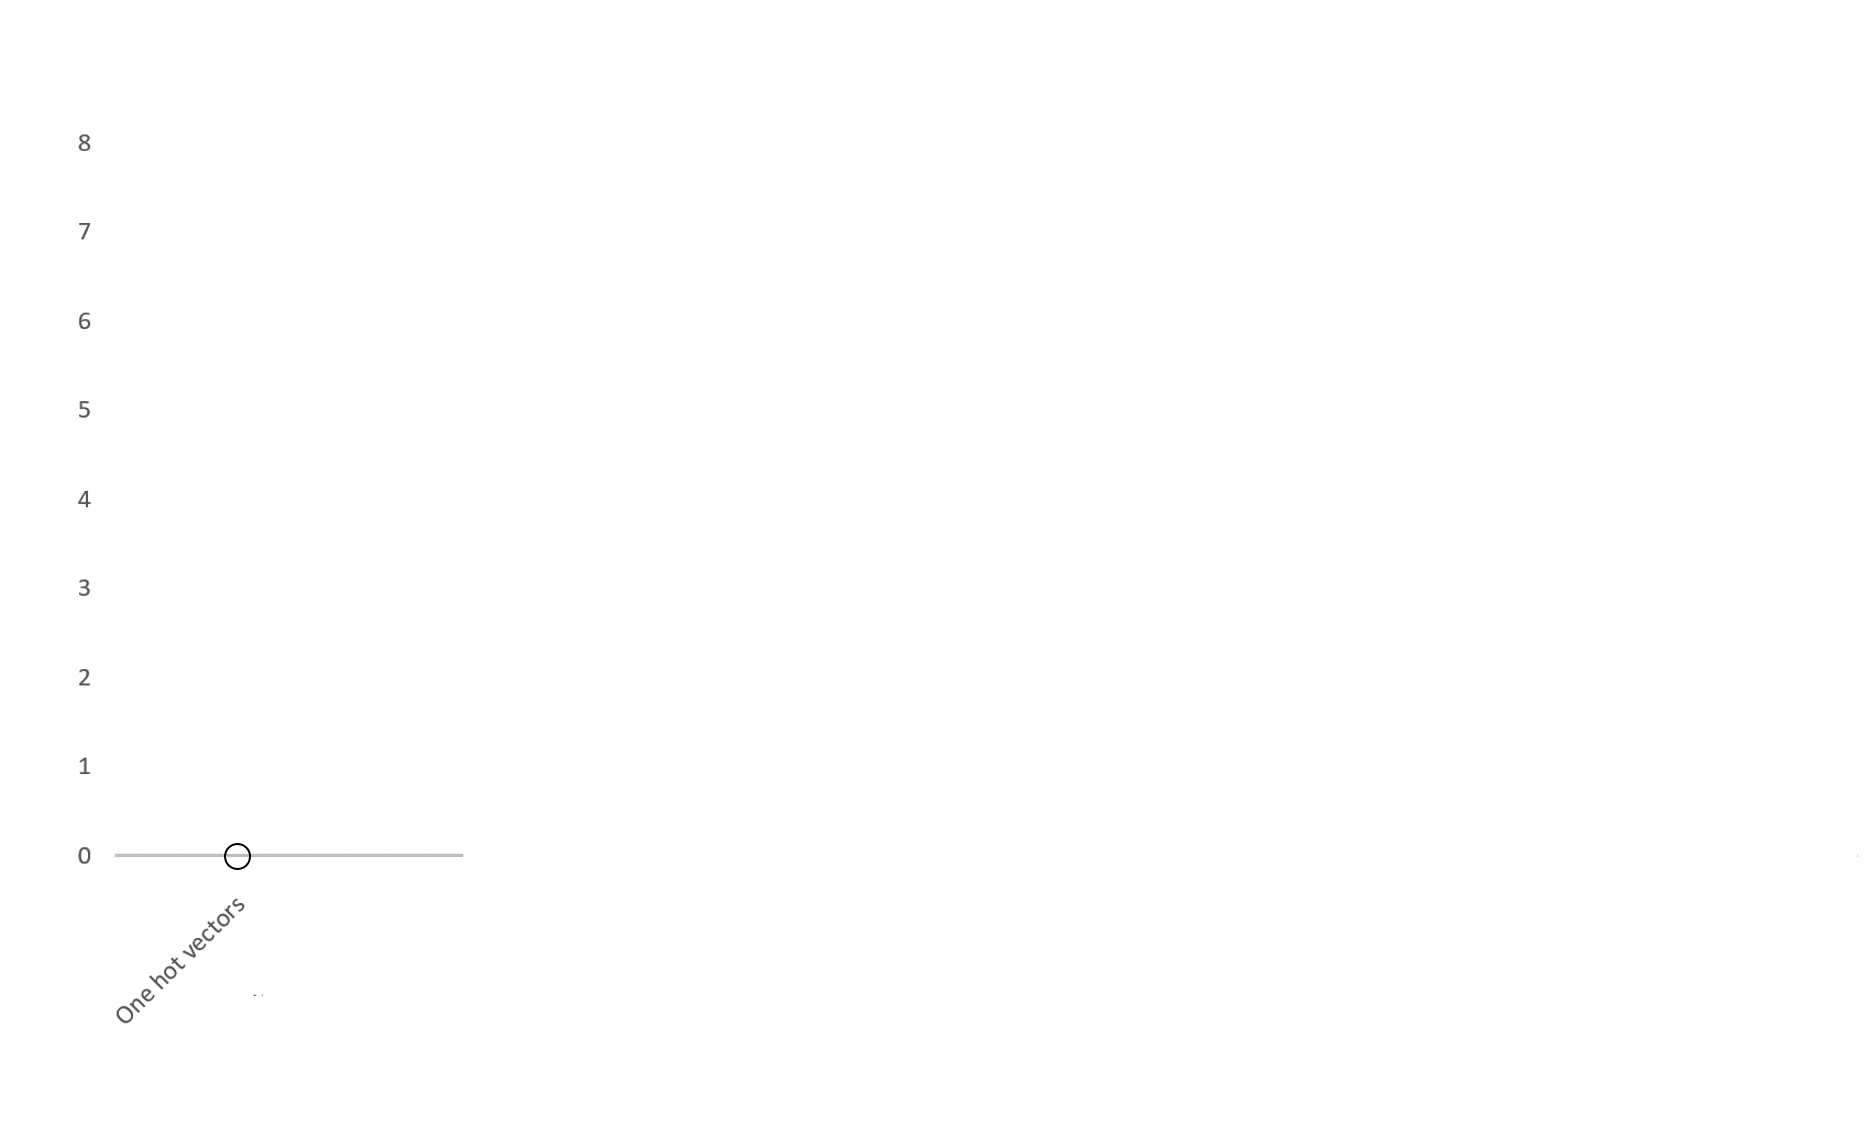
\includegraphics[width=\linewidth,keepaspectratio]{murthy1}

% {\tiny (Ref: Understanding ``Understanding language'' - Murthy Kolluru}

% \end{center}

% \end{frame}


%%%%%%%%%%%%%%%%%%%%%%%%%%%%%%%%%%%%%%%%%%%%%%%%%%%%%%%%%%%%%%%%%%%%%%%%%%%%%%%%%%
\begin{frame}[fragile]\frametitle{Count Vector for Document}
\begin{itemize}
\item Corpus:
\begin{itemize}
\item D1: He is a lazy boy. She is also lazy.
\item D2: Neeraj is a lazy person.
\end{itemize}
\item Dictionary is a list of unique tokens(words) =['He','She','lazy','boy','Neeraj','person'] 
\item Count Matrix:
\begin{center}
\includegraphics[width=\linewidth,keepaspectratio]{word29}
\end{center}
\end{itemize}
\end{frame}

%%%%%%%%%%%%%%%%%%%%%%%%%%%%%%%%%%%%%%%%%%%%%%%%%%%%%%%%%%%%%%%%%%%%%%%%%%%%%%%%%%
\begin{frame}[fragile]\frametitle{Count Vector for Document}
\begin{center}
\includegraphics[width=0.8\linewidth,keepaspectratio]{word30}
\end{center}
\end{frame}


% %%%%%%%%%%%%%%%%%%%%%%%%%%%%%%%%%%%%%%%%%%%%%%%%%%%%%%%%%%%%%%%%%%%%%%%%%%%%%%%%%%
% \begin{frame}[fragile]\frametitle{Murthy's Visualization}

% \begin{center}
% 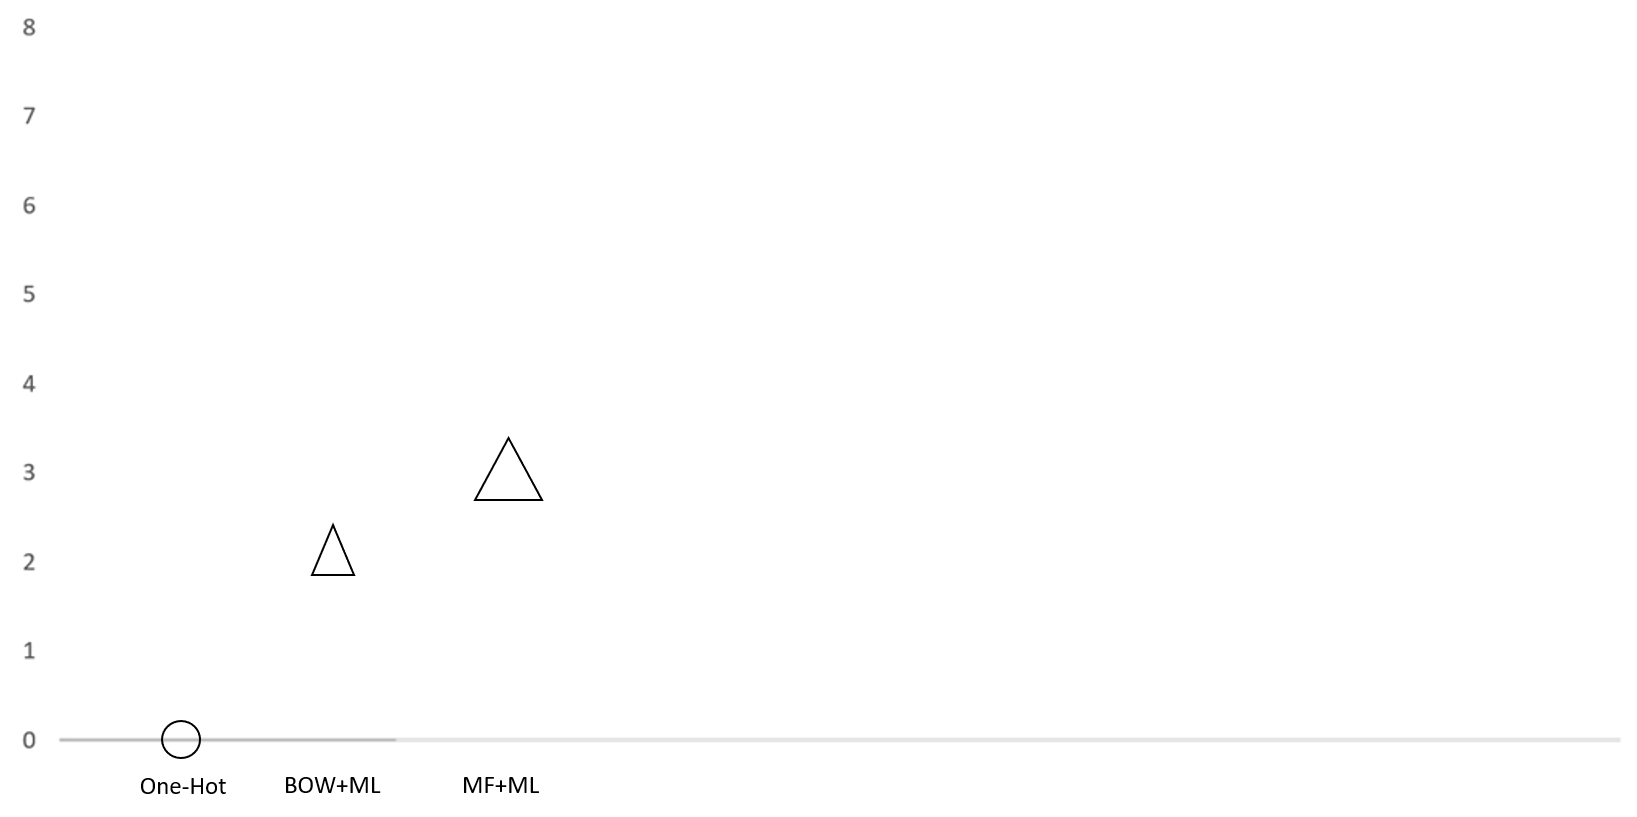
\includegraphics[width=\linewidth,keepaspectratio]{murthy2}

% {\tiny (Ref: Understanding ``Understanding language'' - Murthy Kolluru}

% \end{center}

% \end{frame}

%%%%%%%%%%%%%%%%%%%%%%%%%%%%%%%%%%%%%%%%%%%%%%%%%%%%%%%%%%%%%%%%%%%%%%%%%%%%%%%%%%
\begin{frame}[fragile]\frametitle{TF-IDF Transform}
  \begin{itemize}
    % \item Related to one-hot encoded vectors
	\item Words are represented by their term frequency multiplied by their inverse document frequency.
	\item Words that occur a lot but everywhere should be given very little weighting or significance. 
	\item It takes into account not just the occurrence of a word in a single document but in the entire corpus.
\item Down weigh the common words occurring in almost all documents and give more importance to words that appear in a subset of documents.
  \end{itemize}
  
\begin{center}
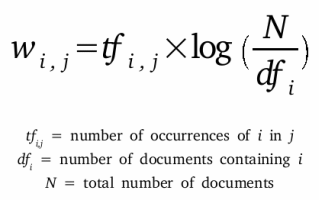
\includegraphics[width=0.5\linewidth,keepaspectratio]{tfidf1}
\end{center}

\end{frame}


%%%%%%%%%%%%%%%%%%%%%%%%%%%%%%%%%%%%%%%%%%%%%%%%%%%%%%%%%%%%%%%%%%%%%%%%%%%%%%%%%%
\begin{frame}[fragile]\frametitle{TF-IDF vectorization}
\begin{itemize}
\item TF = (Number of times term t appears in a document)/(Number of terms in the document)
\item So, TF(This,Document1) = 1/8  and TF(This, Document2)=1/5
\item IDF = log(N/n), where, N is the number of documents and n is the number of documents a term t has appeared in.
\item So, IDF(This) = log(2/2) = 0.
\item TFIDF = TF*IDF
\item Dictionary is made of a list of unique tokens(words) 
\item Similar to Count Matrix, TFIDF matrix is made with TFIDF values in it.
\end{itemize}
\end{frame}


%%%%%%%%%%%%%%%%%%%%%%%%%%%%%%%%%%%%%%%%%%%%%%%%%%%%%%%%%%%%%%%%%%%%%%%%%%%%%%%%%%
\begin{frame}[fragile]\frametitle{TF-IDF Transform}
  \begin{itemize}
	\item Words like ``the'' or ``and'' don't provide a large amount of value.
	\item  However, if a word appears very little or appears frequently, but only in one or two places, then its Imp and should be weighted High.
  \end{itemize}
  
\begin{center}
\includegraphics[width=0.6\linewidth,keepaspectratio]{w2v2}
\end{center}


\end{frame}

%%%%%%%%%%%%%%%%%%%%%%%%%%%%%%%%%%%%%%%%%%%%%%%%%%%%%%%%%%%%%%%%%%%%%%%%%%%%%%%%%%
\begin{frame}[fragile]\frametitle{TF-IDF Inferencing}
Once tf-idf model is trained on a corpus of documents, what happens when a test word or a document is given? How does it calculate tf-idf vector for it?
\begin{itemize}
\item For just one test word, its tf would be 1, then do we just mulitply idf of that word from trained model? Are tf values in trained model irrelevant?
\item Even for test document, does \lstinline|inverse_transform| take into account tfs of current test document or tfs within trained model?
\item Answer: the test word or document is 'ADDED' to the corpus are retraining/calculation is done to arrive at meaningful numbers.
\end{itemize}

{\tiny (Ref: https://stackoverflow.com/questions/55707577/how-does-tfidfvectorizer-compute-scores-on-test-data )}
\end{frame}

%%%%%%%%%%%%%%%%%%%%%%%%%%%%%%%%%%%%%%%%%%%%%%%%%%%%%%%%%%%%%%%%%%%%%%%%%%%%%%%%%%
\begin{frame}[fragile]\frametitle{Problems}
\begin{itemize}
\item This suffers from the downside of very high dimensional representations that don’t capture semantic relatedness.
\item Unable to capture the word meaning.
% \item Corpus:
% \begin{center}
% \includegraphics[width=0.8\linewidth,keepaspectratio]{word31}
% \end{center}
\end{itemize}
\end{frame}



% %%%%%%%%%%%%%%%%%%%%%%%%%%%%%%%%%%%%%%%%%%%%%%%%%%%%%%%%%%%%%%%%%%%%%%%%%%%%%%%%%%
% \begin{frame}[fragile]\frametitle{Co-Occurrence Matrix}
% \begin{itemize}
% \item Co-occurrence ' For a given corpus, the co-occurrence of a pair of words say w1 and w2 is the number of times they have appeared together in a Context Window.
% \item Context Window ' Context window is specified by a number and the direction. So what does a context window of 2 (around) means?
% \begin{center}
% \includegraphics[width=0.6\linewidth,keepaspectratio]{word32}
% \end{center}
% \item For Corpus ='' He is not lazy. He is intelligent. He is smart.''
% \end{itemize}
% \begin{center}
% \includegraphics[width=0.5\linewidth,keepaspectratio]{word33}
% \end{center}
% \end{frame}

% %%%%%%%%%%%%%%%%%%%%%%%%%%%%%%%%%%%%%%%%%%%%%%%%%%%%%%%%%%%%%%%%%%%%%%%%%%%%%%%%%%
% \begin{frame}[fragile]\frametitle{Co-Occurrence Matrix}
% Red box- It is the number of times 'He' and 'is' have appeared in the context window 2 and it can be seen that the count turns out to be 4. 
% \begin{center}
% \includegraphics[width=0.5\linewidth,keepaspectratio]{word34}
% \end{center}
% While the word 'lazy' has never appeared with'intelligent' in the context window and therefore has been assigned 0 in the blue box.
% \end{frame}





%%%%%%%%%%%%%%%%%%%%%%%%%%%%%%%%%%%%%%%%%%%%%%%%%%%%%%%%%%%%%%%%%%%%%%%%%%%%%%%%%%
\begin{frame}[fragile]\frametitle{Good Vector Representation}
\begin{itemize}
\item Traditional One Hot Encoding:
	\begin{itemize}
	\item Apple = [1, 0, 0]
	\item Orange = [0, 1, 0]
	\item Plane = [0, 0, 1]
	\end{itemize}
\begin{center}
\includegraphics[width=0.8\linewidth,keepaspectratio]{word23_1}
\end{center}
\item Very few cells participate in the representation.
\end{itemize}

Whats the solution? \ldots the 'Context'
\end{frame}

%%%%%%%%%%%%%%%%%%%%%%%%%%%%%%%%%%%%%%%%%%%%%%%%%%%%%%%%%%%%%%%%%%%%%%%%%%%%%%%%%%
\begin{frame}[fragile]\frametitle{}

\begin{center}
{\Large Context}
\end{center}
\end{frame}

%%%%%%%%%%%%%%%%%%%%%%%%%%%%%%%%%%%%%%%%%%%%%%%%%%%%%%%%%%%%%%%%%%%%%%%%%%%%%%%%%%
\begin{frame}[fragile]\frametitle{How?}

How to capture context? 
\begin{itemize}
\item Distributional Embeddings enable word vectors to encapsulate contextual context. 
\item Each embedding vector is represented based on the mutual information it has with other words in a given corpus. 
\end{itemize}

Example?
\end{frame}




%%%%%%%%%%%%%%%%%%%%%%%%%%%%%%%%%%%%%%%%%%%%%%%%%%%%%%%%%%%%%%%%%%%%%%%%%%%%%%%%%%
\begin{frame}[fragile]\frametitle{But, What is ``meaning''?}
What is ``bardiwac''?

Anyone?
\end{frame}

%%%%%%%%%%%%%%%%%%%%%%%%%%%%%%%%%%%%%%%%%%%%%%%%%%%%%%%%%%%%%%%%%%%%%%%%%%%%%%%%%%
\begin{frame}[fragile]\frametitle{Lets try again, with examples}
What is ``bardiwac''?

\begin{itemize}
\item He handed her a glass of \underline{bardiwac}. 
\item Beef dishes are made to complement the \underline{bardiwac}.
\item Nigel staggered to his feet, face flushed from too much
\underline{bardiwac}. 
\item Malbec, one of the lesser-known \underline{bardiwac} grapes,
responds well to Australia’s sunshine. 
\item I dined off bread and cheese and this excellent \underline{bardiwac}. 
\item The drinks were delicious: blood-red \underline{bardiwac} as well as 
light, sweet Rhenish. 
\end{itemize}

Now, anyone?
\end{frame}

%%%%%%%%%%%%%%%%%%%%%%%%%%%%%%%%%%%%%%%%%%%%%%%%%%%%%%%%%%%%%%%%%%%%%%%%%%%%%%%%%%
\begin{frame}[fragile]\frametitle{At least one can guess now}
What is ``bardiwac''?

``Bardiwac is a red 
alcoholic beverage 
made from grapes ''

Context helps \ldots
\end{frame}

%%%%%%%%%%%%%%%%%%%%%%%%%%%%%%%%%%%%%%%%%%%%%%%%%%%%%%%%%%%%%%%%%%%%%%%%%%%%%%%%%%
\begin{frame}[fragile]\frametitle{Distributed Semantics/Meaning}
\begin{itemize}
\item  A bottle of \underline{bardiwac} is on the table. 
\item  Everybody likes \underline{bardiwac}.
\item  Don’t have \underline{bardiwac} before you drive. 
\item  We make \underline{bardiwac}  out of corn. 

\end{itemize}
\end{frame}

%%%%%%%%%%%%%%%%%%%%%%%%%%%%%%%%%%%%%%%%%%%%%%%%%%%%%%%%%%%%%%%%%%%%%%%%%%%%%%%%%%
\begin{frame}[fragile]\frametitle{Distributed Semantics/Meaning}
\begin{itemize}
\item  A bottle of \underline{xxxxxxxx} is on the table. 
\item  Everybody likes \underline{xxxxxxxx}.
\item  Don’t have \underline{xxxxxxxx} before you drive. 
\item  We make \underline{xxxxxxxx}  out of corn. 

\end{itemize}

What other words fit into these places? 

Won't they be similar to bardiwac?
\end{frame}

%%%%%%%%%%%%%%%%%%%%%%%%%%%%%%%%%%%%%%%%%%%%%%%%%%%%%%%%%%%%%%%%%%%%%%%%%%%%%%%%%%
\begin{frame}[fragile]\frametitle{Distributed Semantics/Meaning}
\begin{center}
\includegraphics[width=\linewidth,keepaspectratio]{emb6}
\end{center}

{\tiny (Ref: Word Embeddings - Elena Voita, Yandex Research}
\end{frame}



%%%%%%%%%%%%%%%%%%%%%%%%%%%%%%%%%%%%%%%%%%%%%%%%%%%%%%%%%%%%%%%%%%%%%%%%%%%%%%%%%%
\begin{frame}[fragile]\frametitle{Distributed Semantics/Meaning}
Closer ones are \ldots

\begin{center}
\includegraphics[width=0.8\linewidth,keepaspectratio]{emb8}
\end{center}

{\tiny (Ref: Word Embeddings - Elena Voita, Yandex Research)}
\end{frame}


%%%%%%%%%%%%%%%%%%%%%%%%%%%%%%%%%%%%%%%%%%%%%%%%%%%%%%%%%%%%%%%%%%%%%%%%%%%%%%%%%%
\begin{frame}[fragile]\frametitle{Distributed Semantics/Meaning}
Idea of Co-occurance counts \ldots

\begin{center}
\includegraphics[width=0.4\linewidth,keepaspectratio]{emb9}
\end{center}

{\tiny (Ref: Word Embeddings - Elena Voita, Yandex Research)}
\end{frame}

%%%%%%%%%%%%%%%%%%%%%%%%%%%%%%%%%%%%%%%%%%%%%%%%%%%%%%%%%%%%%%%%%%%%%%%%%%%%%%%%%%
\begin{frame}[fragile]\frametitle{Distributed Semantics/Meaning}
Calculate Co-occurrences for the context word, that itself becomes its own representation!!!

\begin{center}
\includegraphics[width=\linewidth,keepaspectratio]{emb10}
\end{center}

{\tiny (Ref: Word Embeddings - Elena Voita, Yandex Research)}
\end{frame}



% %%%%%%%%%%%%%%%%%%%%%%%%%%%%%%%%%%%%%%%%%%%%%%%%%%%%%%%%%%%%%%%%%%%%%%%%%%%%%%%%%%
% \begin{frame}[fragile]\frametitle{Examples}
% \begin{center}
% \includegraphics[width=\linewidth,keepaspectratio]{word12}
% \end{center}
% \end{frame}

% %%%%%%%%%%%%%%%%%%%%%%%%%%%%%%%%%%%%%%%%%%%%%%%%%%%%%%%%%%%%%%%%%%%%%%%%%%%%%%%%%%
% \begin{frame}[fragile]\frametitle{Murthy's Visualization}

% \begin{center}
% 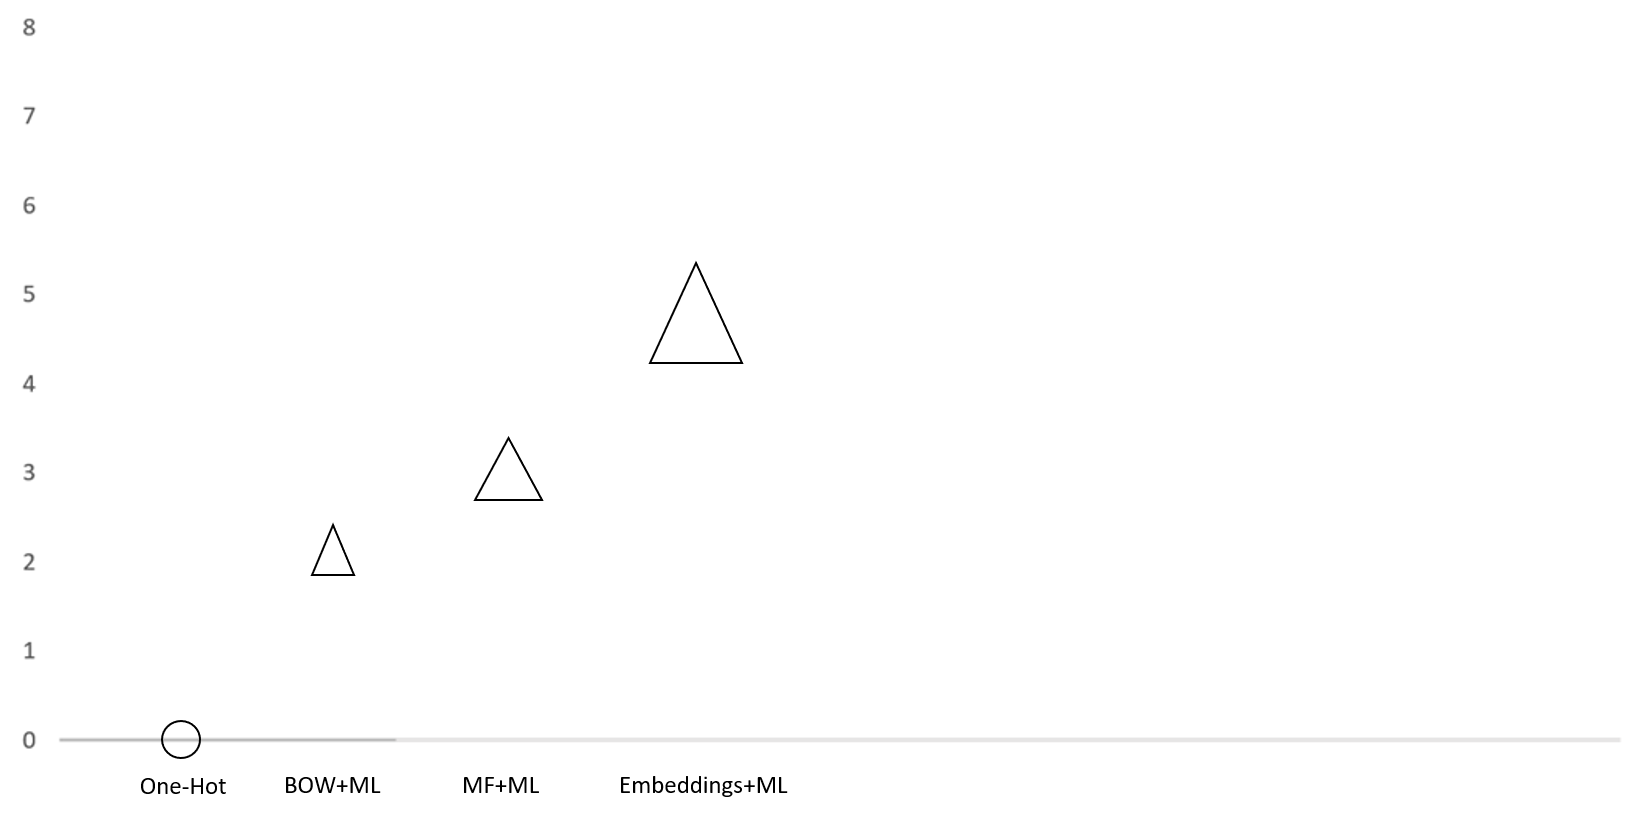
\includegraphics[width=\linewidth,keepaspectratio]{murthy3}

% {\tiny (Ref: Understanding ``Understanding language'' - Murthy Kolluru}

% \end{center}

% \end{frame}

%%%%%%%%%%%%%%%%%%%%%%%%%%%%%%%%%%%%%%%%%%%%%%%%%%%%%%%%%%%%%%%%%%%%%%%%%%%%%%%%%%
\begin{frame}[fragile]\frametitle{}

\begin{center}
{\Large Modern Word Vectors}
\end{center}
\end{frame}




%%%%%%%%%%%%%%%%%%%%%%%%%%%%%%%%%%%%%%%%%%%%%%%%%%%%%%%%%%%%%%%%%%%%%%%%%%%%%%%%%%
\begin{frame}[fragile]\frametitle{Modern Word Vectors}
\begin{itemize}
\item How do we actually build these super-intelligent vectors, that seem to have such magical powers?
\item How to find a word's friends?
\item We will discuss the most famous methods to build such lower-dimension vector representations for words based on their context
\begin{itemize}
% \item Co-occurrence Matrix with SVD
\item Word2vec  (Google)
\item Global Vector Representations (GloVe)   (Stanford)
\item \ldots
\end{itemize}
\end{itemize}
\end{frame}

% %%%%%%%%%%%%%%%%%%%%%%%%%%%%%%%%%%%%%%%%%%%%%%%%%%%%%%%%%%%%%%%%%%%%%%%%%%%%%%%%%%
% \begin{frame}[fragile]\frametitle{Co-occurrence Matrix}
% Co-occurrence Matrix with Singular Value Decomposition:
% \begin{center}
% \includegraphics[width=0.5\linewidth,keepaspectratio]{word16}
% \end{center}
% \end{frame}


% %%%%%%%%%%%%%%%%%%%%%%%%%%%%%%%%%%%%%%%%%%%%%%%%%%%%%%%%%%%%%%%%%%%%%%%%%%%%%%%%%%
% \begin{frame}[fragile]\frametitle{Building a co-occurrence matrix}
% \begin{lstlisting}
% Corpus =  {``I like deep learning''
	    % ``I like NLP''
	    % ``I enjoy flying''} 
% \end{lstlisting}
% \begin{center}
% \includegraphics[width=\linewidth,keepaspectratio]{word17}
% \end{center}
% Context =  previous word and next word
% \end{frame}

% %%%%%%%%%%%%%%%%%%%%%%%%%%%%%%%%%%%%%%%%%%%%%%%%%%%%%%%%%%%%%%%%%%%%%%%%%%%%%%%%%%
% \begin{frame}[fragile]\frametitle{Dimension Reduction using Singular Value Decomposition}
% \begin{center}
% \includegraphics[width=\linewidth,keepaspectratio]{word18}
% \end{center}
% \end{frame}

% %%%%%%%%%%%%%%%%%%%%%%%%%%%%%%%%%%%%%%%%%%%%%%%%%%%%%%%%%%%%%%%%%%%%%%%%%%%%%%%%%%
% \begin{frame}[fragile]\frametitle{Singular Value Decomposition}
% \begin{center}
% \includegraphics[width=\linewidth,keepaspectratio]{word19}
% \end{center}
% The problem with this method, is that we may end up with matrices having billions of rows and columns, which makes SVD computationally restrictive.

% \end{frame}



% %%%%%%%%%%%%%%%%%%%%%%%%%%%%%%%%%%%%%%%%%%%%%%%%%%%%%%%%%%%%%%%%%%%%%%%%%%%%%%%%%
% \begin{frame}[fragile]\frametitle{Language Model }
% \begin{itemize}
% \item A good statistical model for NLP is the conditional probability of the next word w given its previous ones
% \item Takes advantage of both word order, and the fact that temporally closer words have a stronger dependency.
% \end{itemize}

% \end{frame}




%%%%%%%%%%%%%%%%%%%%%%%%%%%%%%%%%%%%%%%%%%%%%%%%%%%%%%%%%%%%%%%%%%%%%%%%%%%%%%%%%%
\begin{frame}[fragile]\frametitle{Word2Vec}
Word2vec  (Google): a distributed representation of a word is used and not sparse like One-Hot.
\begin{center}
\includegraphics[width=0.8\linewidth,keepaspectratio]{word41}
\end{center}
Represent in some abstract way the `meaning' of a word.

\end{frame}

%%%%%%%%%%%%%%%%%%%%%%%%%%%%%%%%%%%%%%%%%%%%%%%%%%%%%%%%%%%%%%%%%%%%%%%%%%%%%%%%%%
\begin{frame}[fragile]\frametitle{Word Distributed Representation - Word2Vec}
\begin{itemize}
\item All vector cells participate in representing each word.
\item Words are represented by real valued dense vectors of significantly smaller dimensions (e.g. 100 - 1000).
\item  Intuition: consider each vector cell as a representative of some feature.
\begin{center}
\includegraphics[width=\linewidth,keepaspectratio]{word24}
\end{center}
\end{itemize}
\end{frame}


%%%%%%%%%%%%%%%%%%%%%%%%%%%%%%%%%%%%%%%%%%%%%%%%%%%%%%%%%%%%%%%%%%%%%%%%%%%%%%%%%%
\begin{frame}[fragile]\frametitle{Word2Vec}
Two major learning approaches:
  \begin{itemize}
    \item Continuous Bag-of-Words (CBOW): Learns an embedding by predicting the current words based on the context. The context is determined by the surrounding words.
	\item Continuous Skip-Gram: Learns an embedding by predicting the surrounding words given the context. The context is the current word.
  \end{itemize}
  
\begin{center}
\includegraphics[width=0.7\linewidth,keepaspectratio]{w2v4}
\end{center}

\end{frame}

%%%%%%%%%%%%%%%%%%%%%%%%%%%%%%%%%%%%%%%%%%%%%%%%%%%%%%%%%%%%%%%%%%%%%%%%%%%%%%%%%%
\begin{frame}[fragile]\frametitle{CBOW}
  
\begin{center}
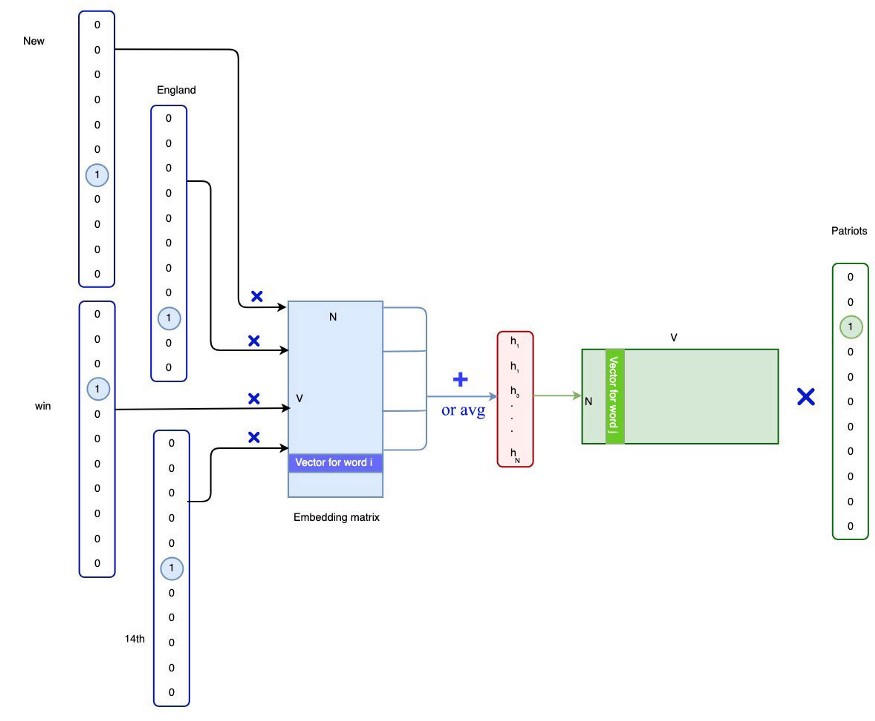
\includegraphics[width=0.7\linewidth,keepaspectratio]{cbow1}
\end{center}

{\tiny (Ref:NLP — Word Embedding \& GloVe - Jonathan Hui )}

\end{frame}


%%%%%%%%%%%%%%%%%%%%%%%%%%%%%%%%%%%%%%%%%%%%%%%%%%%%%%%%%%%%%%%%%%%%%%%%%%%%%%%%%%
\begin{frame}[fragile]\frametitle{Skip-Gram}
  
\begin{center}
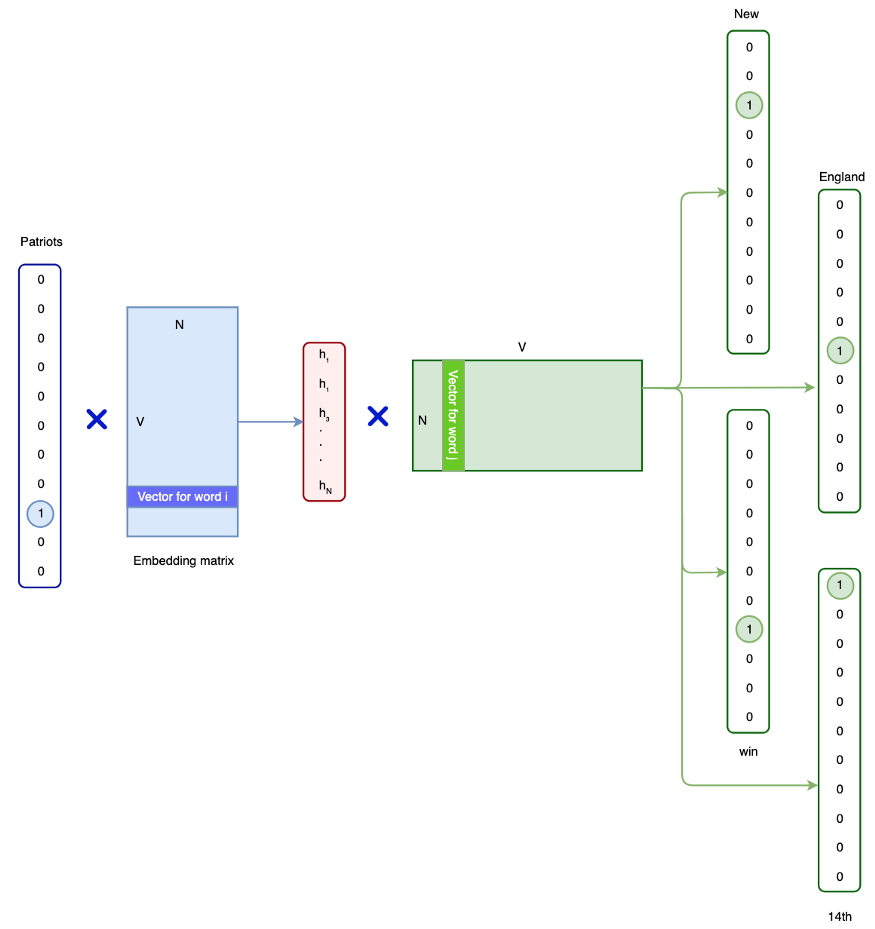
\includegraphics[width=0.6\linewidth,keepaspectratio]{skipgram1}
\end{center}

{\tiny (Ref:NLP — Word Embedding \& GloVe - Jonathan Hui )}

\end{frame}



% %%%%%%%%%%%%%%%%%%%%%%%%%%%%%%%%%%%%%%%%%%%%%%%%%%%%%%%%%%%%%%%%%%%%%%%%%%%%%%%%%
% \begin{frame}[fragile]\frametitle{Google's Word2Vec}
% \begin{itemize}
% \item Continues Bag - of - Words (CBOW): predicts a word given its context (bidirectional).
% \item Skip - Gram: predicts the context given a word (bidirectional).
% \end{itemize}
% \begin{center}
% \includegraphics[width=0.6\linewidth,keepaspectratio]{word25}
% \end{center}
% (Ref: Distributed Representations of Words and Phrases and their Compositionality. Mikolov at al., 2013)
% \end{frame}

%%%%%%%%%%%%%%%%%%%%%%%%%%%%%%%%%%%%%%%%%%%%%%%%%%%%%%%%%%%%%%%%%%%%%%%%%%%%%%%%%%
\begin{frame}[fragile]\frametitle{Word2Vec}
  \begin{itemize}
    \item Both of these learning methods use local word usage context (with a defined window of neighboring words). 
	\item The larger the window is, the more topical similarities that are learned by the embedding. Forcing a smaller window results in more semantic, syntactic, and functional similarities to be learned.
  \end{itemize}

\end{frame}

%%%%%%%%%%%%%%%%%%%%%%%%%%%%%%%%%%%%%%%%%%%%%%%%%%%%%%%%%%%%%%%%%%%%%%%%%%%%%%%%%%
\begin{frame}[fragile]\frametitle{Benefits}
  \begin{itemize}
    \item Low space and low time complexity to generate a rich representation
	\item The larger the dimensionality, the more features we can have in our representation
	\item Allows us to efficiently generate something like a billion word corpora, 
	\item But encompass a bunch of generalities and keep the dimensionality small.
  \end{itemize}

\end{frame}

% %%%%%%%%%%%%%%%%%%%%%%%%%%%%%%%%%%%%%%%%%%%%%%%%%%%%%%%%%%%%%%%%%%%%%%%%%%%%%%%%%%
% \begin{frame}[fragile]\frametitle{Word2Vec}
% \begin{center}
% \includegraphics[width=\linewidth,keepaspectratio]{word20}
% \end{center}
% \end{frame}

% %%%%%%%%%%%%%%%%%%%%%%%%%%%%%%%%%%%%%%%%%%%%%%%%%%%%%%%%%%%%%%%%%%%%%%%%%%%%%%%%%
% \begin{frame}[fragile]\frametitle{Word2Vec Architecture}
% \begin{center}
% \includegraphics[width=0.8\linewidth,keepaspectratio]{word21}
% \end{center}
% \end{frame}


% %%%%%%%%%%%%%%%%%%%%%%%%%%%%%%%%%%%%%%%%%%%%%%%%%%%%%%%%%%%%%%%%%%%%%%%%%%%%%%%%%
% \begin{frame}[fragile]\frametitle{Context windows}
% \begin{itemize}
% \item Context can be anything - a surrounding n-gram, a randomly sampled set of words from a fixed size window around the word
% \item For example, assume context is defined as the word following a word. $context(w_i) = w_{i+1}$
% \item Corpus :  I ate the cat
% \item Training Set  : $I|ate,  ate|the ,  the|cat, cat|. $
% \end{itemize}
% \end{frame}


% %%%%%%%%%%%%%%%%%%%%%%%%%%%%%%%%%%%%%%%%%%%%%%%%%%%%%%%%%%%%%%%%%%%%%%%%%%%%%%%%%%
% \begin{frame}[fragile]\frametitle{Google's Word2Vec}
% \begin{center}
% \includegraphics[width=\linewidth,keepaspectratio]{emb11}
% \end{center}

% {\tiny (Ref: Word Embeddings - Elena Voita, Yandex Research)}
% \end{frame}


%%%%%%%%%%%%%%%%%%%%%%%%%%%%%%%%%%%%%%%%%%%%%%%%%%%%%%%%%%%%%%%%%%%%%%%%%%%%%%%%%%
\begin{frame}[fragile]\frametitle{Glove}
  \begin{itemize}
    % \item An extension of word2vec, and a much better one at that.
	% \item Contribution was the addition of global statistics in the language modeling task to generate the embedding. 
	\item There is no window feature for local context like Word2Vec
	\item Glove uses Global context, across the entire corpora.
	\item Uses co-occuring matrix based distributional embeddings,
	\item Uses neural methods to decompose the co-occurrence matrix into more expressive and dense word vectors.
  \end{itemize}
  
\begin{center}
\includegraphics[width=0.9\linewidth,keepaspectratio]{w2v5}
\end{center}
  
\end{frame}

% %%%%%%%%%%%%%%%%%%%%%%%%%%%%%%%%%%%%%%%%%%%%%%%%%%%%%%%%%%%%%%%%%%%%%%%%%%%%%%%%%%
% \begin{frame}[fragile]\frametitle{FastText}
  % \begin{itemize}
    % \item To incorporate sub-word information by splitting all words into a bag of n-gram characters (typically of size 3-6). 
	% \item It would add these sub-words together to create a whole word as a final feature. 
	% \item Power: support out-of-vocabulary words! 
	% \item n other approaches, if the system encounters a word that it doesn’t recognize, it just has to set it to the unknown word. With FastText, we can give meaning to words like circumnavigate if we only know the word navigate, because our semantic knowledge of the word navigate can help use at least provide a bit more semantic information to circumnavigate, even if it is not a word our system learned during training.
  % \end{itemize}
  
 
% \end{frame}

% %%%%%%%%%%%%%%%%%%%%%%%%%%%%%%%%%%%%%%%%%%%%%%%%%%%%%%%%%%%%%%%%%%%%%%%%%%%%%%%%%%
% \begin{frame}[fragile]\frametitle{FastText}
  % \begin{itemize}
    % \item Uses the skip-gram objective with negative sampling. 
	% \item All sub-words are positive examples, and then random samples from a dictionary of words in the corpora are used as negative examples.
	% \item Facebook, in developing FastText, has published pre-trained FastText vectors in 294 different languages.
  % \end{itemize}
  
 
% \end{frame}

% %%%%%%%%%%%%%%%%%%%%%%%%%%%%%%%%%%%%%%%%%%%%%%%%%%%%%%%%%%%%%%%%%%%%%%%%%%%%%%%%%%
% \begin{frame}[fragile]\frametitle{Poincare Embeddings (Hierarchal Representations)}
  % \begin{itemize}
    % \item Use hyperbolic geometry to capture hierarchal properties of words. 
	% \item Hyperbolic space distance to encode similarity and the norm of vectors to encode hierarchal relationships.
	% \item  Less dimensions are needed
  % \end{itemize}
  
 % \begin{center}
% \includegraphics[width=0.6\linewidth,keepaspectratio]{w2v6}
% \end{center}
% \end{frame}

% %%%%%%%%%%%%%%%%%%%%%%%%%%%%%%%%%%%%%%%%%%%%%%%%%%%%%%%%%%%%%%%%%%%%%%%%%%%%%%%%%%
% \begin{frame}[fragile]\frametitle{ELMo}
  % \begin{itemize}
    % \item Generated from a function of the entire sentence to create word-level representations.
	% \item The embeddings are generated at a character-level, so they can capitalize on sub-word units like FastText and do not suffer from the issue of out-of-vocabulary words.
	% \item Trained as a bi-directional, two layer LSTM language model
	% \item Lowest layer is good for things like POS tagging and other more syntactic and functional tasks, whereas the higher layer is good for things like word-sense disambiguation and other higher-level, more abstract tasks.
  % \end{itemize}

% \end{frame}


%%%%%%%%%%%%%%%%%%%%%%%%%%%%%%%%%%%%%%%%%%%%%%%%%%%%%%%%%%%%%%%%%%%%%%%%%%%%%%%%%%
\begin{frame}[fragile]\frametitle{}

\begin{center}
{\Large Examples}
\end{center}
\end{frame}




%%%%%%%%%%%%%%%%%%%%%%%%%%%%%%%%%%%%%%%%%%%%%%%%%%%%%%%%%%%%%%%%%%%%%%%%%%%%%%%%%%
\begin{frame}[fragile]\frametitle{Examples}
Vectors for King, Man, Queen, \& Woman:
\begin{center}
\includegraphics[width=0.5\linewidth,keepaspectratio]{word42}
\end{center}


\begin{center}
\includegraphics[width=0.5\linewidth,keepaspectratio]{word44}
\end{center}

\end{frame}

%%%%%%%%%%%%%%%%%%%%%%%%%%%%%%%%%%%%%%%%%%%%%%%%%%%%%%%%%%%%%%%%%%%%%%%%%%%%%%%%%%
\begin{frame}[fragile]\frametitle{Examples}
Gender relation:
\begin{center}
\includegraphics[width=0.35\linewidth,keepaspectratio]{word45}
\end{center}
Plural relation:

\begin{center}
\includegraphics[width=0.35\linewidth,keepaspectratio]{word46}
\end{center}

\end{frame}


%%%%%%%%%%%%%%%%%%%%%%%%%%%%%%%%%%%%%%%%%%%%%%%%%%%%%%%%%%%%%%%%%%%%%%%%%%%%%%%%%%
\begin{frame}[fragile]\frametitle{Examples}
Word pair relationships:
\begin{center}
\includegraphics[width=0.4\linewidth,keepaspectratio]{word47}
\end{center}
Country-capital city relationship:

\begin{center}
\includegraphics[width=0.4\linewidth,keepaspectratio]{word48}
\end{center}

\end{frame}




%%%%%%%%%%%%%%%%%%%%%%%%%%%%%%%%%%%%%%%%%%%%%%%%%%%%%%%%%%%%%%%%%%%%%%%%%%%%%%%%%%
\begin{frame}[fragile]\frametitle{Word Representations Comparison}

\adjustbox{valign=t}{
\begin{minipage}{0.45\linewidth}
Traditional Method  - Bag of Words Model

\begin{itemize}
\item Uses one hot encoding
\item Each word in the vocabulary is represented by one bit position in a HUGE vector.
\item For example, with a vocabulary of 10000 words, and ''Hello'' is the 4th word in the dictionary:  \lstinline|0 0 0 1 0 0  . . . . . . . 0 0 0 0 |
\item Context information is not utilized
\end{itemize}
\end{minipage}
}
\hfill
\adjustbox{valign=t}{
\begin{minipage}{0.45\linewidth}
Modern - Word Vectors

\begin{itemize}
\item Stores each word in as a point in space, represented by a vector of fixed number of dimensions (generally 300)
\item Unsupervised, built just by reading huge corpus
\item For example, ''Hello'' might be represented as :  \lstinline| [0.4, -0.11, 0.55, 0.3 . . . 0.1, 0.02]|
\item Context information is utilized
\end{itemize}
\end{minipage}
}
\end{frame}




% %%%%%%%%%%%%%%%%%%%%%%%%%%%%%%%%%%%%%%%%%%%%%%%%%%%%%%%%%%%%%%%%%%%%%%%%%%%%%%%%%%
% \begin{frame}[fragile]\frametitle{Probabilistic Graphical Models}
% Markov process based Language Models also capture semantics

% \begin{itemize}
% \item  Hidden Markov models
% \item Conditional Random Fields
% \end{itemize}

% {\tiny (Ref: Understanding ``Understanding language'' - Murthy Kolluru}

% \end{frame}


% %%%%%%%%%%%%%%%%%%%%%%%%%%%%%%%%%%%%%%%%%%%%%%%%%%%%%%%%%%%%%%%%%%%%%%%%%%%%%%%%%%
% \begin{frame}[fragile]\frametitle{Murthy's Visualization}

% \begin{center}
% 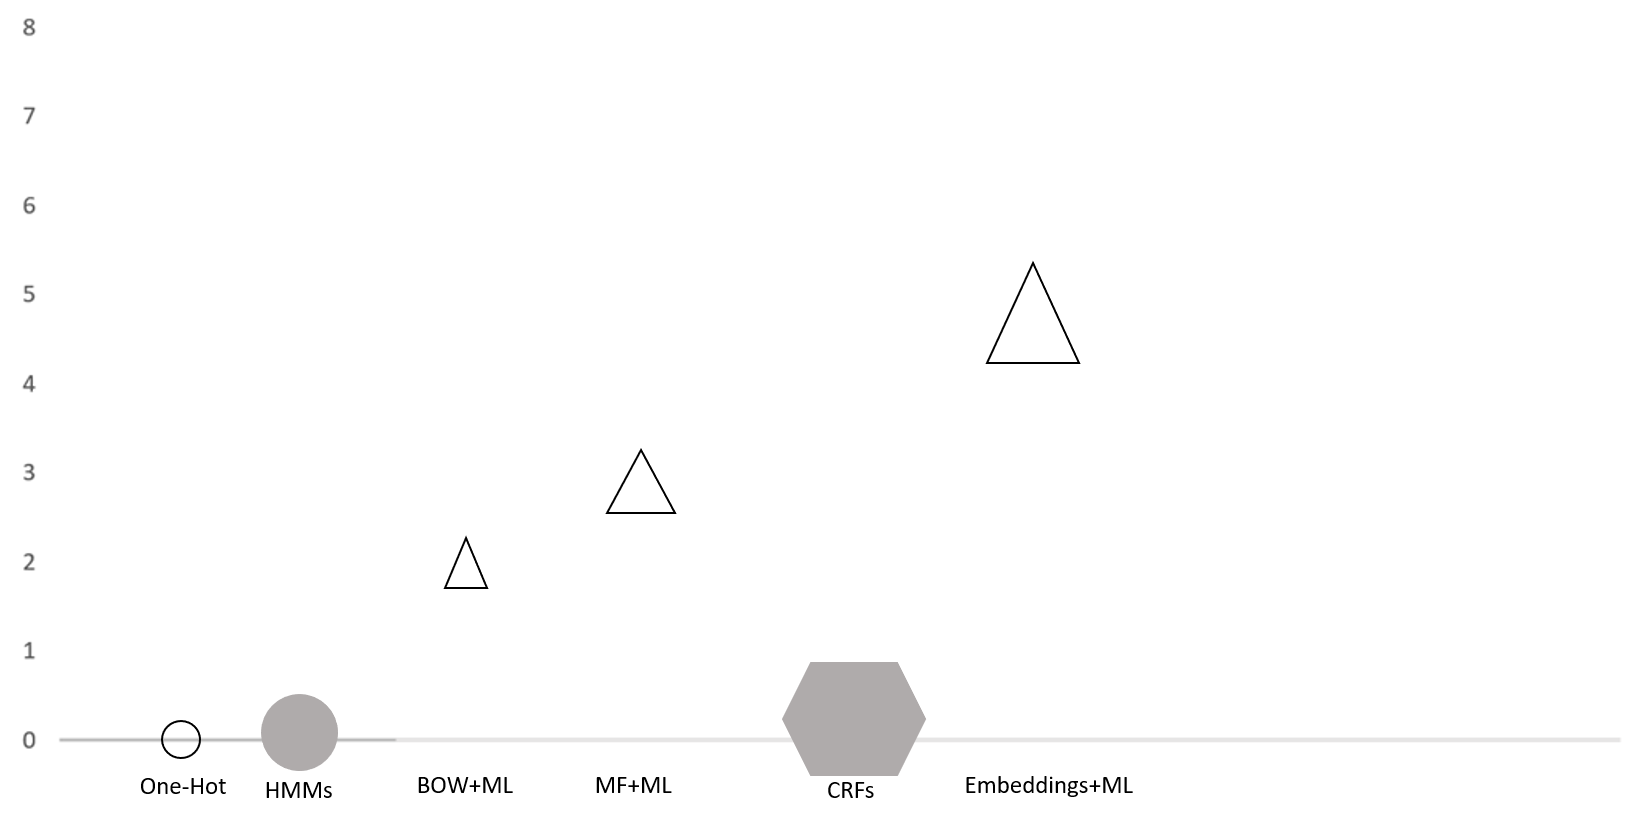
\includegraphics[width=\linewidth,keepaspectratio]{murthy4}

% {\tiny (Ref: Understanding ``Understanding language'' - Murthy Kolluru}

% \end{center}

% \end{frame}



% %%%%%%%%%%%%%%%%%%%%%%%%%%%%%%%%%%%%%%%%%%%%%%%%%%%%%%%%%%%%%%%%%%%%%%%%%%%%%%%%%%
% \begin{frame}[fragile]\frametitle{Transfer learning}
% Very popular in Image processing but a late entry into NLP world

% \begin{itemize}
% \item Pre-train with language models
% \item Train same net on multiple tasks
% \end{itemize}

% {\tiny (Ref: Understanding ``Understanding language'' - Murthy Kolluru}

% \end{frame}

% %%%%%%%%%%%%%%%%%%%%%%%%%%%%%%%%%%%%%%%%%%%%%%%%%%%%%%%%%%%%%%%%%%%%%%%%%%%%%%%%%%
% \begin{frame}[fragile]\frametitle{Murthy's Visualization}

% \begin{center}
% 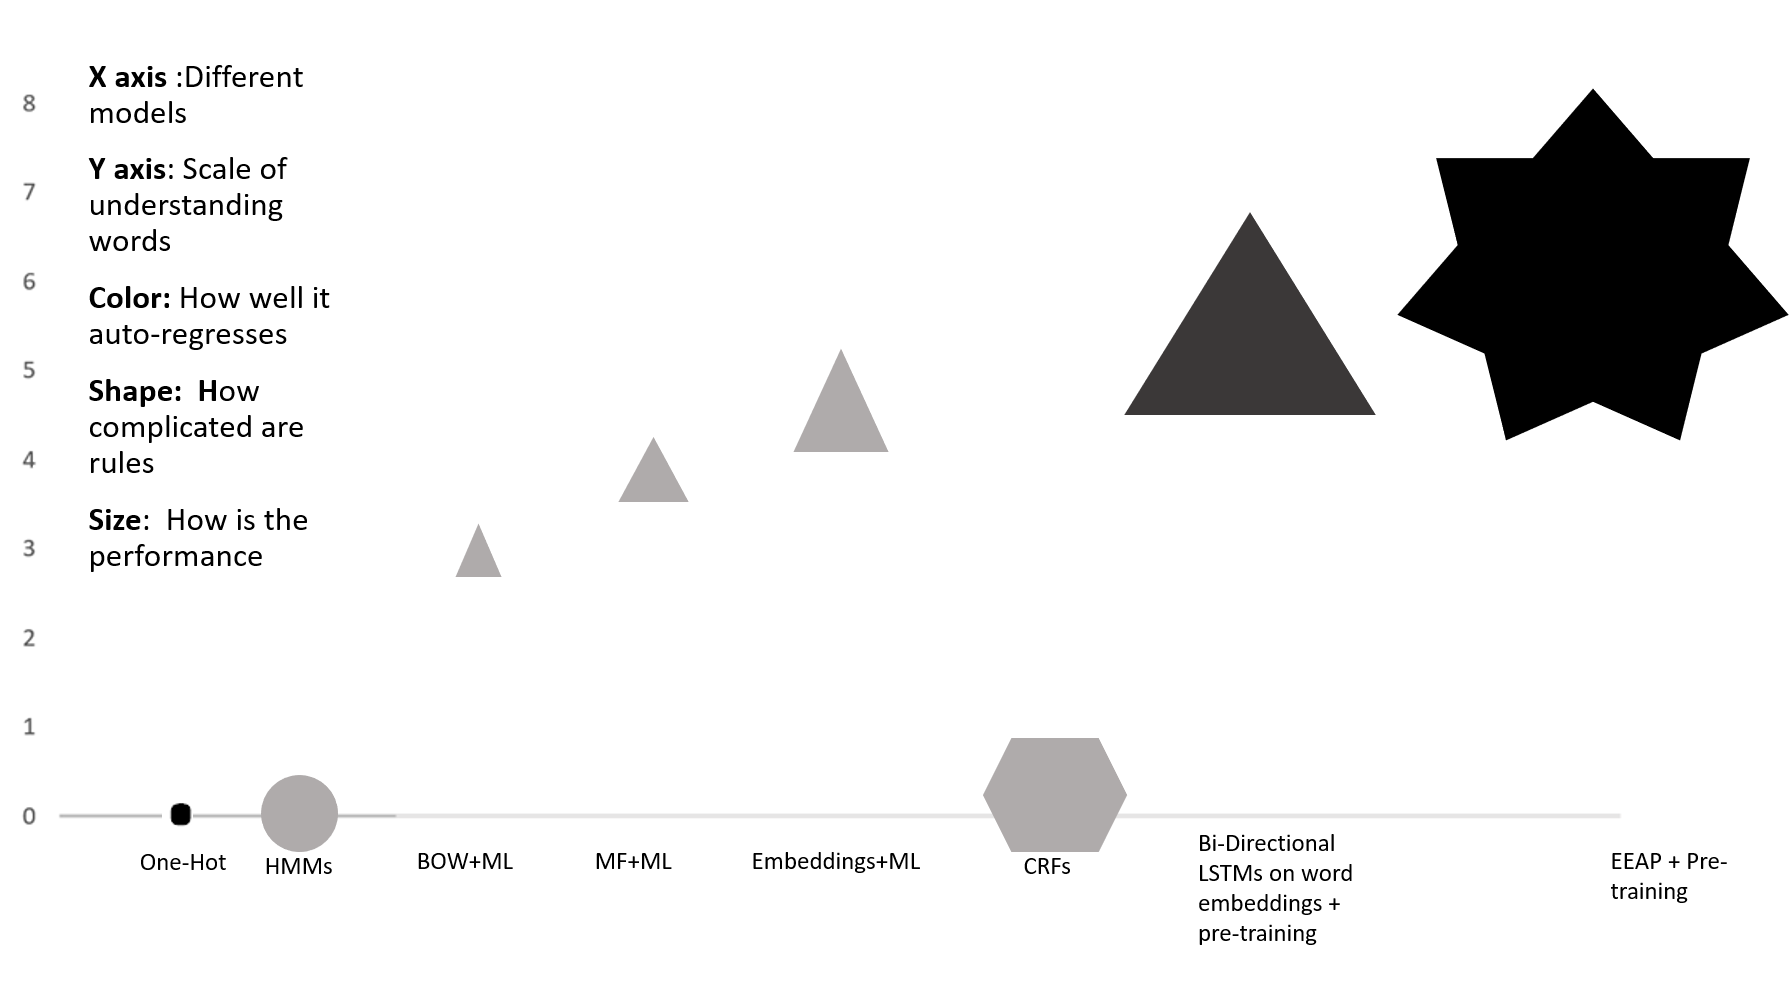
\includegraphics[width=\linewidth,keepaspectratio]{murthy5}

% {\tiny (Ref: Understanding ``Understanding language'' - Murthy Kolluru}

% \end{center}

% \end{frame}

% %%%%%%%%%%%%%%%%%%%%%%%%%%%%%%%%%%%%%%%%%%%%%%%%%%%%%%%%%%%%%%%%%%%%%%%%%%%%%%%%%%
% \begin{frame}[fragile]\frametitle{Murthy's Visualization}

% \begin{center}
% 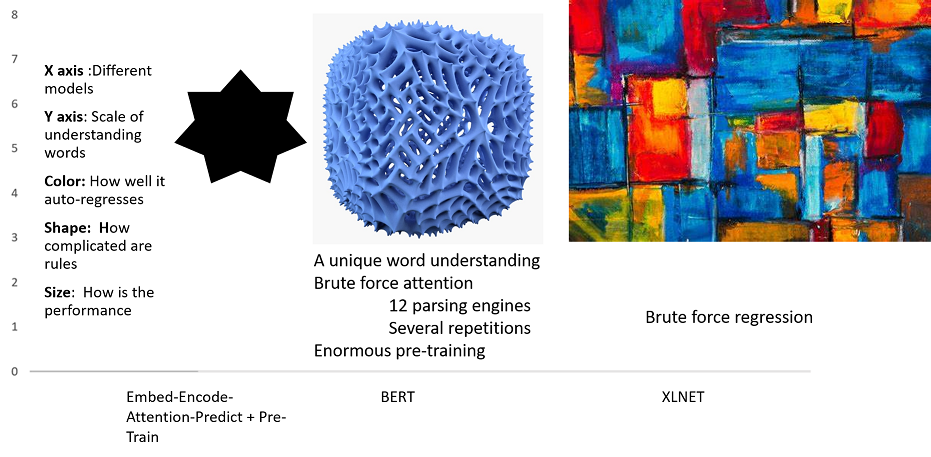
\includegraphics[width=\linewidth,keepaspectratio]{murthy6}

% {\tiny (Ref: Understanding ``Understanding language'' - Murthy Kolluru}

% \end{center}

% \end{frame}

%%%%%%%%%%%%%%%%%%%%%%%%%%%%%%%%%%%%%%%%%%%%%%%%%%%%%%%%%%%%%%%%%%%%%%%%%%%%%%%%%%
\begin{frame}[fragile]\frametitle{}

\begin{center}
{\Large Applications}
\end{center}
\end{frame}




%%%%%%%%%%%%%%%%%%%%%%%%%%%%%%%%%%%%%%%%%%%%%%%%%%%%%%%%%%%%%%%%%%%%%%%%%%%%%%%%%%
\begin{frame}[fragile]\frametitle{Word Similarity}
\begin{itemize}
\item Classic Methods :  Edit Distance, WordNet, Porter's Stemmer, Lemmatization using dictionaries
\item Easily identifies similar words and synonyms since they occur in similar contexts
\item Stemming (thought $\rightarrow$ think) 
\item Inflections, Tense forms
\item eg. Think, thought, ponder, pondering,
\item eg. Plane, Aircraft, Flight
\end{itemize}
\end{frame}


%%%%%%%%%%%%%%%%%%%%%%%%%%%%%%%%%%%%%%%%%%%%%%%%%%%%%%%%%%%%%%%%%%%%%%%%%%%%%%%%%%
\begin{frame}[fragile]\frametitle{Machine Translation}

\begin{itemize}
\item Classic Methods :  Rule-based machine translation, morphological transformation
\begin{center}
\includegraphics[width=0.6\linewidth,keepaspectratio]{word13}
\end{center}
\end{itemize}
\end{frame}

%%%%%%%%%%%%%%%%%%%%%%%%%%%%%%%%%%%%%%%%%%%%%%%%%%%%%%%%%%%%%%%%%%%%%%%%%%%%%%%%%%
\begin{frame}[fragile]\frametitle{Part-of-Speech and Named Entity Recognition}


\begin{itemize}
\item Classic Methods :  Sequential Models (MEMM , Conditional Random Fields),  Logistic Regression
\begin{center}
\includegraphics[width=0.8\linewidth,keepaspectratio]{word10}
\end{center}
\end{itemize}
\end{frame}
%
%%%%%%%%%%%%%%%%%%%%%%%%%%%%%%%%%%%%%%%%%%%%%%%%%%%%%%%%%%%%%%%%%%%%%%%%%%%%%%%%%%%
%\begin{frame}[fragile]\frametitle{Applications of Word Vectors}
%Relation Extraction:
%
%\begin{itemize}
%\item Classic Methods : OpenIE, Linear programing models, Bootstrapping
%\begin{center}
%\includegraphics[width=0.8\linewidth,keepaspectratio]{word11}
%\end{center}
%\end{itemize}
%\end{frame}

%%%%%%%%%%%%%%%%%%%%%%%%%%%%%%%%%%%%%%%%%%%%%%%%%%%%%%%%%%%%%%%%%%%%%%%%%%%%%%%%%%
\begin{frame}[fragile]\frametitle{Sentiment Analysis}

\begin{itemize}
\item Classic Methods : Naive Bayes, Random Forests/SVM
\item Classifying sentences as positive and negative
\item Building sentiment lexicons using seed sentiment sets
\item No need for classifiers, we can just use cosine distances to compare unseen reviews to known reviews.

\begin{center}
\includegraphics[width=0.7\linewidth,keepaspectratio]{word15}
\end{center}
\end{itemize}
\end{frame}

%%%%%%%%%%%%%%%%%%%%%%%%%%%%%%%%%%%%%%%%%%%%%%%%%%%%%%%%%%%%%%%%%%%%%%%%%%%%%%%%%%
\begin{frame}[fragile]\frametitle{Other Applications}
\begin{itemize}
\item Co-reference Resolution: Chaining entity mentions across multiple documents  - can we find and unify the multiple contexts in which mentions occurs?
\item Clustering: Words in the same class naturally occur in similar contexts,  and this feature vector can directly be used with any conventional clustering algorithms (K-Means, agglomerative, etc). Human doesn't have to waste time hand-picking useful word features to cluster on.
\item Topic modeling: Semantic Analysis of Documents: Build word distributions for various topics, etc.

\end{itemize}
\end{frame}

%%%%%%%%%%%%%%%%%%%%%%%%%%%%%%%%%%%%%%%%%%%%%%%%%%%%%%%%%%%%%%%%%%%%%%%%%%%%%%%%%%
\begin{frame}[fragile]\frametitle{}

\begin{center}
{\Large Evaluation}
\end{center}
\end{frame}


%%%%%%%%%%%%%%%%%%%%%%%%%%%%%%%%%%%%%%%%%%%%%%%%%%%%%%%%%%%%%%%%%%%%%%%%%%%%%%%%%%
\begin{frame}[fragile]\frametitle{Efficacy}
Intrinsic: evaluation on a specific/intermediate subtask
\begin{itemize}
\item  word analogies: “a is to b as c is to \underline{xxxx}?” 
\item  word similarity: correlation of the rankings
\end{itemize}
Extrinsic: evaluation on a real task
\begin{itemize}
\item  take some task (MT, NER, coreference resolution, …) or several tasks
\item   train with different pretrained word embeddings
\item  if the task quality is better -> win!
\end{itemize}
\end{frame}

%%%%%%%%%%%%%%%%%%%%%%%%%%%%%%%%%%%%%%%%%%%%%%%%%%%%%%%%%%%%%%%%%%%%%%%%%%%%%%%%%%
\begin{frame}[fragile]\frametitle{Domain Understanding}
  \begin{itemize}
    \item Another big advantage is that  is that we can actually pre-train word embeddings that are applicable to many tasks. 
	\item Only caution is that these embeddings are generic text corpus and carry general meanings.
	\item If you want domain specific meanings, then you will need to build your own word embeddings.
	\item ``Shell'' in zoology could mean creature houses you find on sea shore, but the same word in CAD means Hollowing operation.
	\item ``Draft'' in legal domain is a rough document, where as in CAD it is Tapering operation.
  \end{itemize}



\end{frame}


%%%%%%%%%%%%%%%%%%%%%%%%%%%%%%%%%%%%%%%%%%%%%%%%%%%%%%%%%%%%%%%%%%%%%%%%%%%%%%%%%%
\begin{frame}[fragile]\frametitle{Advantages}

\begin{itemize}
\item They provide a fresh perspective to ALL  problems in NLP, and not just solve one problem.
\item Technological Improvement
\item Rise of deep learning since 2006 (Big Data + GPUs  + Work done by Andrew Ng, Yoshua Bengio, Yann Lecun and Geoff Hinton)
\item Application of Deep Learning to NLP - led by Yoshua Bengio,  Christopher Manning, Richard Socher, Tomas Mikalov
\item The need for unsupervised learning . (Supervised learning tends to be excessively dependent on hand-labeled data and often does not scale)
\end{itemize}
\end{frame}



%%%%%%%%%%%%%%%%%%%%%%%%%%%%%%%%%%%%%%%%%%%%%%%%%%%%%%%%%%%%%%%%%%%%%%%%%%%%%%%%%%
\begin{frame}[fragile]\frametitle{Disadvantages}
\begin{itemize}
\item Single vector for a word (whats problem with that?)
\item Very vulnerable, and not a robust concept
\item Can take a long time to train
\item Non-uniform results
\item Hard to understand and visualize
\end{itemize}
\end{frame}

%%%%%%%%%%%%%%%%%%%%%%%%%%%%%%%%%%%%%%%%%%%%%%%%%%%%%%%%%%%%%%%%%%%%%%%%%%%%%%%%%%
\begin{frame}[fragile]\frametitle{}

\begin{center}
{\Large Conclusion}
\end{center}
\end{frame}


%%%%%%%%%%%%%%%%%%%%%%%%%%%%%%%%%%%%%%%%%%%%%%%%%%%%%%%%%%%%%%%%%%%%%%%%%%%%%%%%%%
\begin{frame}[fragile]\frametitle{What is a word embedding?}
\begin{itemize}
\item Word Embeddings are the texts converted into numbers
\item There may be different numerical representations of  same text. 
\item Many Machine Learning algorithms and almost all Deep Learning Architectures are incapable of processing strings or plain text in their raw form. 
\item They require numbers as inputs to perform any sort of job, be it classification, regression etc. in broad terms.
\item So, for the computer to be able to ''understand'' a vector representation of a word is required.
\end{itemize}
\end{frame}


%%%%%%%%%%%%%%%%%%%%%%%%%%%%%%%%%%%%%%%%%%%%%%%%%%%%%%%%%%%%%%%%%%%%%%%%%%%%%%%%%%
\begin{frame}[fragile]\frametitle{Captures Relationship}
  \begin{itemize}
    \item Word embedding = vector representation of a word
	\item A word is `embedded' in $n$ dimensional space.
	\item Once the words are vectors, their prosperities can be utilized.
	\item One such property is dot product giving cosine similarity.
	\item Goal is to capture some sort of relationship in that space, be it meaning, morphology, context, or some other kind of relationship.
  \end{itemize}


\end{frame}

%%%%%%%%%%%%%%%%%%%%%%%%%%%%%%%%%%%%%%%%%%%%%%%%%%%%%%%%%%%%%%%%%%%%%%%%%%%%%%%%%%
\begin{frame}[fragile]\frametitle{Domains}
  \begin{itemize}
    \item The choice of $n$ in word embedding space, is our choice.
	\item It can be tens or hundreds instead of millions (like one-hot encoded vectors).
	\item A lot of word embeddings are created based on the notion introduced by Zellig Harris'``distributional hypothesis'' which boils down to a simple idea that words that are used close to one another typically have the same meaning.
	\item Different word embeddings are created either in different ways or using different text corpora to map this distributional relationship
  \end{itemize}


\end{frame}


%%%%%%%%%%%%%%%%%%%%%%%%%%%%%%%%%%%%%%%%%%%%%%%%%%%%%%%%%%%%%%%%%%%%%%%%%%%%%%%%%%
\begin{frame}[fragile]\frametitle{What Next?}
Machines like humans need four things to understand language

\begin{itemize}
\item Understand the words (semantics)
\item Build the ability to guess (language model)
\item Parse language specific rules and patterns (encoder-decoder, transformers)
\item Build on the experience (pre-training)
\end{itemize}

Ability to include non-language information (culture, visuals, etc) will improve language models.

\end{frame}